\documentclass[conference]{IEEEtran}
\IEEEoverridecommandlockouts
% The preceding line is only needed to identify funding in the first footnote. If that is unneeded, please comment it out.
\usepackage{cite}
\usepackage{amsmath,amssymb,amsfonts}
\usepackage{algorithmic}
\usepackage{graphicx}
\usepackage{textcomp}
\usepackage{xcolor}
\usepackage{url}
\def\BibTeX{{\rm B\kern-.05em{\sc i\kern-.025em b}\kern-.08em
    T\kern-.1667em\lower.7ex\hbox{E}\kern-.125emX}}
\begin{document}

\title{Day Ahead Load Forecasting for the Modern Distribution Network - A Tasmanian Case Study}

\author{\IEEEauthorblockN{Michael Jurasovic}
\IEEEauthorblockA{\textit{School of Engineering} \\
\textit{University of Tasmania}\\
Hobart, Australia \\
mjj4@utas.edu.au}
\and
\IEEEauthorblockN{Evan Franklin}
\IEEEauthorblockA{\textit{School of Engineering} \\
\textit{University of Tasmania}\\
Hobart, Australia \\
evan.franklin@utas.edu.au
}
\and
\IEEEauthorblockN{Michael Negnevitsky}
\IEEEauthorblockA{\textit{School of Engineering} \\
\textit{University of Tasmania}\\
Hobart, Australia \\
michael.negnevitsky@utas.edu.au}
\and
\IEEEauthorblockN{Paul Scott}
\IEEEauthorblockA{\textit{Research School of Computer Science} \\
\textit{Australian National University}\\
Canberra, Australia \\
paul.scott@anu.edu.au}
}

\maketitle

\begin{abstract}
Just gonna reserve some space for the abstract.
The transformer neural network architecture was applied to short term load forecasting.
The transformer neural network architecture was applied to short term load forecasting.
The transformer neural network architecture was applied to short term load forecasting.
The transformer neural network architecture was applied to short term load forecasting.
The transformer neural network architecture was applied to short term load forecasting.
The transformer neural network architecture was applied to short term load forecasting.
The transformer neural network architecture was applied to short term load forecasting.
The transformer neural network architecture was applied to short term load forecasting.
The transformer neural network architecture was applied to short term load forecasting.
The transformer neural network architecture was applied to short term load forecasting.
The transformer neural network architecture was applied to short term load forecasting.
The transformer neural network architecture was applied to short term load forecasting.
\end{abstract}

\begin{IEEEkeywords}
load forecasting, neural network, machine learning, DER
\end{IEEEkeywords}

\section{Introduction}
Electricity distribution networks, and the way in which they are managed, are currently going through a significant transition, with perhaps more change over the last ten years than in the previous hundred. %the sort of statement where a ref would help strengthen it, but OK not to have
Until recently, generation and load were largely viewed and managed separately: power was produced almost exclusively by large, centralised generating units, and was consumed by customers after \textbf{reticulation} via %traversing is not quite right word. reticulation... hmm???
the transmission and distribution networks. 
Networks were designed and built for demand profiles which were relatively stable over time, with demand forecasting at distribution feeder level required primarily for network planning purposes only. 
Increasingly, power is both consumed by customers connected to the distribution network and is also generated and manipulated by distributed energy resources (DER) within the distribution network, often behind the meter of individual consumers. 
The impact of increasing levels of DER in the system creates, among other things, both a need and an opportunity to more actively manage distribution networks, while also resulting in a generally less predictable net demand profile.

DERs are controllable devices in the power network that generate, store, and/or consume power. 
This includes solar photovoltaic generation (PV), battery storage, and electric vehicles. 
In Australia, the dominant DER technology deployed to date is solar PV, with over 1.8 million systems now reportedly installed on residential properties \textbf{[Ref APVI]}. 
It is widely anticipated that battery storage and electrical vehicle uptake may be just as rapid \textbf{[BNEF Ref]}.

The Tasmanian distribution network, meanwhile, is forecast to experience significant increases in these technologies by 2025: \\
\begin{itemize}
	\item 1500\% increase in battery storage capacity (from 5MWh to 75MWh) \cite{Jacobs2017}
	\item 170\% increase in PV installation capacity (from 130MW to 220MW) \cite{Jacobs2017}
	\item 39\% of new car sales will be EVs - the highest in the country \cite{AEMO2016}
\end{itemize}

The changing nature of the distribution network presents an opportunity to maximize the use of existing assets by delaying the need for network augmentations, while also providing customers with a more reliable supply of power.
For example, batteries could be used to peak-shift, reducing maximum feeder load.
However, to achieve this reliably and with optimal use of available DER generally requires sophisticated methods to optimize the power flow to and from the distributed resources.

\begin{figure}[htbp]
	\centerline{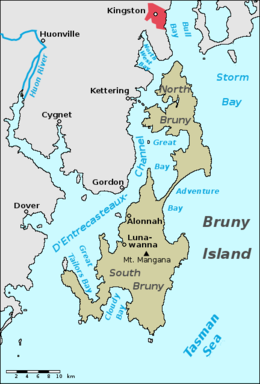
\includegraphics[width=.35\textwidth]{images/bruny_island_map.png}}
	\caption{Bruny Island in southeast Tasmania experiences significant increases in load during holiday periods and was used as a case study for the load forecaster.}
	\label{fig:bruny_map}
\end{figure}

One method to achieve this coordination of DER in distribution networks is presented in \cite{Scott2014} and has been implemented on Bruny Island, Tasmania as part of the CONSORT project.
Bruny Island, shown in Figure \ref{fig:bruny_map}, is a popular holiday destination and during peak periods - such as Easter morning and afternoon peaks - the submarine feeder supplying the island becomes overloaded and has to be supplemented by a diesel generator located on the island.
The aim of the CONSORT project was to effectively peak shift the load away from the morning and afternoon peaks to prevent the use of the generator.

To fulfil such an objective while using the available distributed resources optimally, the CONSORT project relies upon having an accurate, online, 24-hour horizon forecast at the feeder level.
Load forecasting methods commonly employed in industry are neither intended to forecast with high accuracy over a time period this short nor at such a low level in the distribution network \cite{CIGRE2016}.
An improved method for producing accurate feeder-level forecasts is not only highly desirable for this project, but will also in future become a critical element of active distribution network management more generally.

In this paper, a novel neural network-based day-ahead feeder level load forecasting system is developed, with its performance evaluated using ten years of historical demand data for training and testing. We implement the forecast live on Tasmania's Bruny Island distribution network, enabling the CONSORT project's residential battery systems to effectively support the network during periods of peak demand on the network.

\section{Forecasting System Architecture}
Recurrent Neural Networks (RNN) have recently been popular for load forecasting in electricity networks \cite{Kong2018}.
However, RNNs have been out-performed by the Transformer \cite{Vaswani2017} model in several domains including machine translation \cite{Vaswani2017} (where the architecture was first proposed and applied), medical time series forecasting and regression \cite{Song2017}, and image generation \cite{Parmar2018}.
\par
The proposed forecasting system uses a Transformer neural network model combined with similar load profile selection.
The basis for the Transformer model is... \textbf{add a descriptive sentence}
\par
Given a multivariate time series $X = (\boldsymbol{x}_1, ..., \boldsymbol{x}_P)$, with $\boldsymbol{x}_t \in \mathbb{R}^S$ denoting a point in time comprised of $S$ observations (a single point in an S-variate time series), the forecasting system produces a univariate time series forecast $Y = (\boldsymbol{y}_1, ..., \boldsymbol{y}_R)$ with $\boldsymbol{y}_t \in \mathbb{R}^1$.
\par
The points in $X$ and $Y$ are evenly spaced, e.g. 30 or 60 minutes apart, and this is the same for both $X$ and $Y$.
$X$ and $Y$ are aligned on any five minute interval, allowing the forecast to be updated every five minutes.


\subsection{Similar Load Profile Selection}
\textbf{add a sentence at the start explaining why you have this section, what the relevance is etc.}
A load profile \textbf{(profile for short)} is a time series of electrical load over some period of time.
In this paper, all profiles are measured in kVA and are univariate. 

Load profiles are influenced by exogenous factors such as weather, day of the week, and holiday type \cite{Weron2006}.
Holiday type indicates which holiday the profile occurs on - Easter or Christmas for example.
These different holidays are assigned different integer identifiers (with normal days assigned identifier 0) to form a time series.
The forecasting system was provided with historical load and weather profiles that had similar exogenous data to the load profile being forecast.

Similar profiles were identified by first finding candidate similar profiles an integer multiple of 1 year $\pm$30 days away from the profile being forecast and filtering the candidates down to profiles with exactly matching hour and minute.
The hour and minute used were in local time to account for changes around daylight savings.

Then the weighted Euclidean distance between the profile being forecast and each candidate profile was calculated using the following features: 
maximum future temperature, 
minimum future temperature,
maximum past load,
holiday type, 
day of week,
day of month, and
month of year.
When the holiday type always occurs on the same date each year then the month of year and day of month were used, and when the holiday type always occurs on the same day of week each year then the day of week was used.

These features are taken from the model input - thus requiring the model input to contain data from both the past and future if similar profile selection is to be used.
Typically, 24 hours in both directions is used.
The candidate profiles with the lowest distance were selected to be used as input, and their corresponding historical weather data was also supplied as an input.
\par
When training and testing the model the similar days were selected from both the past and the future, as the train and test datasets were only five years each.

\begin{figure}[htbp]
	\centerline{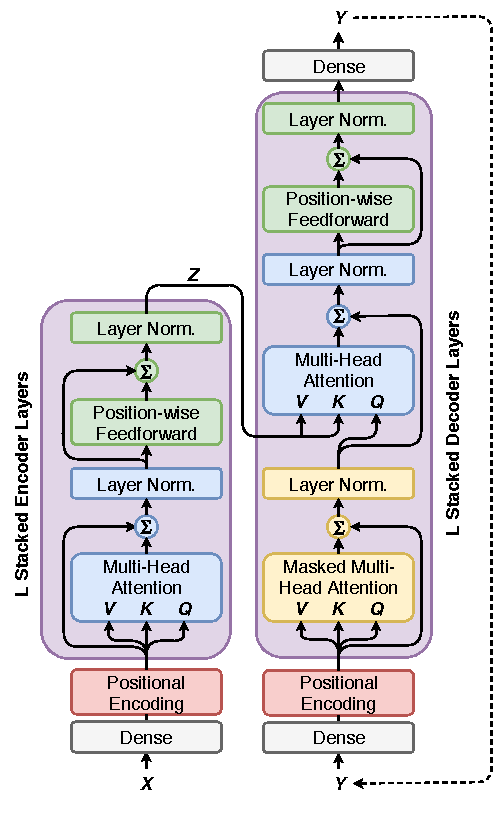
\includegraphics[width=.35\textwidth]{images/transformer.pdf}}
	\caption{The Transformer architecture.}
	\label{fig:transformer}
\end{figure}

\subsection{Transformer}
The transformer neural network architecture, shown in figure \ref{fig:transformer}, was introduced by \cite{Vaswani2017} in 2017 and at the time was the state of the art in neural machine translation.
This architecture follows the standard sequence-to-sequence/encoder-decoder architecture: the encoder transforms an input $X = (\boldsymbol{x}_1, ..., \boldsymbol{x}_P)$ into a latent representation $Z = (\boldsymbol{z}_1, ..., \boldsymbol{z}_Q)$, and the decoder transforms $Z$ into an output sequence $Y = (\boldsymbol{y}_1, ..., \boldsymbol{y}_R)$.

The encoder is constructed of a stack of $L$ identical layers, each containing two sub-layers.
The first is multi-head self-attention and the second is a position-wise feed-foward network, both discussed below.
Both sub-layers have a residual connection around them and are fed into a normalization layer.

The decoder is similar to the encoder except for a third layer which implements multi-head attention on the outputs of the encoder - the attention queries come from the previous decoder layer, while the keys and values come from the encoder output.
The input to the decoder is the previous output of the decoder, but shifted right by one and with every value not yet predicted set to zero.
This requires an iterative approach to be used to predict all points in the time series.
The self-attention in the decoder is masked so that when evaluating a query at time $t$ it is unable to assign large weights to keys/values occurring after $t$ in time - ensuring the decoder is autoregressive.

The individual sections of the transformer are discussed in the following sections.

\subsection{Input Embedding}
The input $\boldsymbol{X} \in \mathbb{R}^{T \times N}$, where the rows represent $T$ points in time and the columns represent $N$ time series, is embedded by applying a dense layer to produce an embedded $\boldsymbol{Y} \in \mathbb{R}^{T \times d}$, with $d$ being the hidden dimension of of the model.
This is intended to allow the neural network to learn the relationships and dependencies between the different input time series.
The embedded representation is given by Equation \ref{dense_layer}, with learned weights $\boldsymbol{W} \in \mathbb{R}^{N \times d}$ and a learned bias vector $\boldsymbol{b} \in \mathbb{R}^{d}$.

\begin{equation} \label{dense_layer}
\boldsymbol{Y} = \text{max}(0, \boldsymbol{XW} + \boldsymbol{b})
\end{equation}

\subsection{Positional Encoding}
The model has no way of telling the position or order of each element in the input, so this information is injected in the positional encoding layer.
This is done by using a learned lookup table to add the same value to the inputs at both test and train time depending on their position in time in the input.
Specifically, a matrix lookup table of embeddings $\boldsymbol{E} \in \mathbb{R}^{T \times d}$ is added to the embedded inputs as per Equation \ref{positional_encoding}.
\begin{equation}\label{positional_encoding}
\boldsymbol{Y} = \boldsymbol{X} + \boldsymbol{E}
\end{equation}

\subsection{Multi-Head Attention} \label{multihead_attention}
The primary innovation of the Transformer architecture is multi-head attention.
Generic attention and dot-product attention will now be described as these are prerequisite to describing multi-head attention.

Given a single query vector and a set of key and value pairs (with each key and each value being a vector), an attention function matches the query to the keys to produce a weight for each key.
These key weights are then used to create an output vector comprised of the weighted sum of the values, where each value's weight is the weight assigned to its corresponding key. 
Matching of the query to the keys is performed with an arbitrary fitness function.

Scaled dot-product attention, shown in Figure \ref{fig:multihead} (left), is a specific implementation of an attention function. 
It uses the dot product of the query and each key to generate the weights, which are then passed through a softmax function such that the sum of all weights is equal to 1.
In practice, the query row vectors are combined into a single matrix, $\boldsymbol{Q}$, allowing computationally cheap matrix calculations to be used to evaluate the attention outputs in parallel.
The keys and values are represented by row vectors in $\boldsymbol{K}$ and $\boldsymbol{V}$, respectively.

The dot product of the keys and queries is scaled (hence the name) by multiplying it by $1 / \sqrt{d_k}$, with $d_k$ being the key and query dimension, to prevent the dot product from becoming large when $d_k$ is large.
A large dot product may cause the gradient of the softmax function to become small and cause issues with training of the model.

The causal mask shown in Figure \ref{fig:multihead} is used exclusively in the decoder self-attention (where $\boldsymbol{Q}$, $\boldsymbol{K}$ and $\boldsymbol{V}$ are identical) to prevent the attention function from matching any query to a key that occurs after itself in time.
This is achieved by leaving the lower triangular portion of the matrix untouched and setting the other values to be large negative numbers - indicating a very poor match.

Multi-head attention, shown in Figure \ref{fig:multihead} (right), applies a separate dense layer to each of the values, queries, and keys. 
The dense layer is applied per Equation \ref{dense_layer} with learned weights $\boldsymbol{W} \in \mathbb{R}^{d \times d}$ and a learned bias vector $\boldsymbol{b} \in \mathbb{R}^{d}$.
The outputs of the dense layers are then split along the last axis into $h$ sets, or heads.
As a result the key, query, and value dimension is reduced by a factor of $h$ to $\frac{d}{h}$.
Scaled dot-product attention is then run independently on each set.
The results are concatenated and put through a final dense layer to produce the output of the attention function.
The dense layer function on the output is defined by Equation \ref{dense_layer} where $\boldsymbol{W} \in \mathbb{R}^{d \times d}$ is a learned weight matrix and $\boldsymbol{b} \in \mathbb{R}^{d}$ is a learned bias vector.

The theory behind multi-head attention is that the dense layer combined with the split allows the model to pick out information from different subspaces in the input and direct these to different attention heads.
This supposedly improves performance over a single head.

\begin{figure}[htbp]
	\centerline{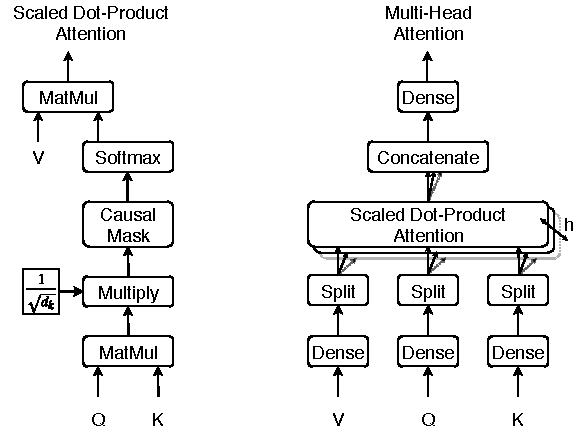
\includegraphics[width=.35\textwidth]{images/multihead_attn.pdf}}
	\caption{Multiheaded attention (right) splits the key, query, and value matrices and applies scaled dot product attention (left) on each in parallel before concatenating the result to return the data to its original dimension.}
	\label{fig:multihead}
\end{figure}

\subsection{Feed-forward}
The feed-forward layer is a two layer network with a rectified linear unit in the middle.
Given an input $\boldsymbol{X} \in \mathbb{R}^{T \times d}$, the output $\boldsymbol{Y} \in \mathbb{R}^{T \times d}$ is populated by Equation \ref{feedforward} where $\boldsymbol{W}_1 \in \mathbb{R}^{d \times 4d}$, $\boldsymbol{b}_1 \in \mathbb{R}^{4d}$, $\boldsymbol{W}_2 \in \mathbb{R}^{4d \times d}$, and $\boldsymbol{b}_2 \in \mathbb{R}^{d}$ are learned weights and biases.

\begin{equation} \label{feedforward}
\boldsymbol{Y} = \text{max}(0, \boldsymbol{X}  \boldsymbol{W}_1 + \boldsymbol{b}_1)  \boldsymbol{W}_2 + \boldsymbol{b}_2
\end{equation}

\subsection{Decoder Dense Output}
The output of the decoder is passed through a dense layer to project the hidden dimension to the desired dimension of 1.
The layer is implemented per Equation \ref{dense_layer} where $\boldsymbol{W} \in \mathbb{R}^{d \times 1}$ is a learned weight matrix and $\boldsymbol{b} \in \mathbb{R}^{1}$ is a learned bias vector.



\subsection{Residuals \& Normalization}
Residual connections \cite{He2015} are applied around each sub-layer.
That is, the output of each sub-layer is given by $\boldsymbol{Y} = \boldsymbol{X} + \text{subLayer}(\boldsymbol{X})$ where subLayer$(\boldsymbol{X})$ is the original output of the sub-layer.
The outputs are then normalized by applying layer normalization \cite{Ba2016}, as per Equation \ref{layernorm} where $\mu_{\boldsymbol{x}}$ and $\sigma_{\boldsymbol{x}}$ are the mean and variance of $\boldsymbol{x}$ respectively.

\begin{equation} \label{layernorm}
\boldsymbol{Y}_{i,*} = \frac{\mu_{\boldsymbol{X}_{i,*}}}{\sigma_{\boldsymbol{X}_{i,*}}}
\end{equation}

\subsection{Dropout and Training}
Dropout is applied during training in the following positions:
\begin{itemize}
	\item At the output of the positional encoding of both the encoder and decoder.
	\item Immediately after the softmax operation in the scaled dot-product attention.
\end{itemize}
The model is trained using the Adam optimizer \cite{Kingma2014}.
The loss function is a modified sum squared error.
Given a vector $\boldsymbol{y}$ of predictions from the model and a vector $\boldsymbol{y'}$ of expected predictions the loss function $l$ is given by 
\begin{equation}
l = \sum_{t=0}^{R}((\boldsymbol{y}_t - \boldsymbol{y'}_t)^2 \times |\boldsymbol{y'}_t|^c)
\end{equation}
Where $c$ is a model hyperparameter.
For $c>0$ this function accentuates loss when the actual value is large - this is useful for a load forecast as times of maximum demand are likely important for planning purposes.
When $c=0$ this is simply normal sum squared error, and for $c<0$ this will accentuate loss when the actual value is small.

When testing or being used for inference, the decoder outputs are generated sequentially one at a time.
After each output value is generated it is shifted right by one and populated in the decoder input and the model is executed again until finally all the outputs have been generated.
Values that have not yet been generated are set to zero in the decoder input.
These zero values do not affect the output of the decoder, as the decoder self-attention is masked so that it does not make use of them.
When training, the decoder input is set to the known expected value and the model is executed a single time.


\section{Case Study}

\subsection{Bruny Island}
Bruny Island, shown in Figure \ref{fig:bruny_map}, is located approximately two kilometres off the coast of south-east Tasmania with a permanent resident population of approximately 800 people \cite{census2016}.
The island is a popular holiday destination, with Easter periods typically experiencing an influx of up to 500 cars in a single day.
The island is supplied by two feeders, depicted in Figure \ref{fig:bruny_network}.
One feeder supplies a small load in the North of the island and the other supplies the main portion of the island to the South - this case study deals only with the feeder supplying the main portion of the island.

During holiday period morning and afternoon peaks the submarine feeder reaches its capacity and a diesel generator located on the island is used to reduce the feeder load.
The substantial increase in load over the Easter holiday period can be seen in Figure \ref{fig:bruny_easter}.

To avoid the use of the generator, the CONSORT project installed a set of residential batteries on the island for the purposes of peak-shifting.
These batteries are coordinated by the network aware coordination algorithm (NAC).
In order to peak-shift while making efficient use of the batteries, the NAC requires an accurate forecast of load with a 24-hour horizon and 30-minute resolution.
The proposed architecture was implemented for this purpose.

\begin{figure}[htbp]
	\centerline{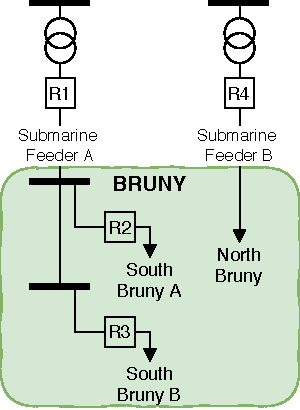
\includegraphics[width=.2\textwidth]{images/bruny_single_line.pdf}}
	\caption{Single line schematic of distribution network on Bruny Island.
			 The majority of load is in the South of the island, fed from submarine feeder A, while a small load is supplied in the North by submarine feeder B}
	\label{fig:bruny_network}
\end{figure}

\begin{figure}[htbp]
	\centerline{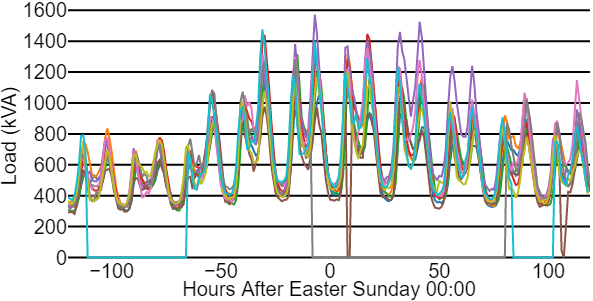
\includegraphics[width=.35\textwidth]{images/easter_bruny.png}}
	\caption{Easters on Bruny Island 2008 through 2017. All Easter Sundays are aligned.}
	\label{fig:bruny_easter}
\end{figure}

\subsection{Data and  Model Configuration}
The following data was available from 2009-2018:
\begin{itemize}
	\item Apparent power at reclosers R1 through R4 (Figure \ref{fig:bruny_network}).
	\item Temperature at Lenah Valley, Tasmania (50km from Bruny Island). 
	\item Apparent power consumption at St Helens, Tasmania.
\end{itemize}

This data was averaged to 30 minute resolution and split into a training set containing data from October 2009 through September 2014, and a testing set containing data from October 2014 through April 2018.

The network was supplied with data from the previous and future 24 hours, for a total input sequence length of 96 (representing 48 hours at 30 minute resolution).
The output sequence length was 48 (24 hours).

The following time series were supplied as input to the model:
\begin{itemize}
	\item Apparent power from recloser R1, with future values set to zero.
	\item Temperature.
	\item Day of the week as an integer from 0 to 6 (local time).
	\item Minutes since midnight (local time).
	\item Boolean 1 or 0 indicating whether it is a holiday.
	\item Holiday type.
\end{itemize}

The source of the temperature data was Lenah Valley for testing and training, whereas for inference it was from the historical and forecast data for Bruny Island from the Bureau of Meteorology.

Additionally, five similar days were identified using data from R1.
The data corresponding to the similar days from each of the following time series was provided as input:
\begin{itemize}
	\item Reclosers R1, R2, R3, and R4 (as separate time series).
	\item St Helens recloser.
	\item Lenah Valley temperature.
\end{itemize}

In total, 36 time series were provided as input to the model.
The data from St Helens was included because it was observed to display similar patterns to Bruny Island around holiday periods.
It was theorized that it may provide additional information to the model, while also serving as a proof of concept for the ability to supply arbitrary exogenous data to the model.

If any value in an input or expected output sequence was bad or missing then the sequence was not used.
As a result, approximately 4\% of the data was discarded.
All data was normalized between zero and one prior to being supplied to the model.
Additionally, the encoder inputs, decoder inputs and expected outputs were summed with randomly distributed noise with a mean of 0 and standard deviation of 0.01 before being supplied to the model.

The forecasting system was configured with the parameters in table \ref{table:parameters}, with the upper section giving transformer model parameters and the lower section giving weights used for similar load profile selection.

\begin{table}[htbp]
	\caption{Case study model parameters}
	\begin{center}
		\begin{tabular}{clc}
%			3.\hline
			\textbf{Parameter}&\textbf{Description}&\textbf{Value} \\
			\hline
			$L$ & Number of encoder and decoder layers & 4 \\
			$d$ & Hidden dimension & 32 \\
			$h$ & Number of attention heads & 4 \\
			$D$ & Dropout fraction & 0.2 \\
			$c$ & Loss function modifier & 3 \\
			-   & Training batch size & 16 \\
			\hline
			-   & Maximum future temperature weight & 10 \\
			-   & Minimum future temperature weight & 20 \\
			-   & Maximum past load weight & 30 \\
			-   & Holiday type weight & 1e9 \\
			-   & Day of week weight & 1e6 \\
			-   & Day of month weight & 1e6 \\
			-   & Month of year weight & 1e6 \\
			
		\end{tabular}
		\label{table:parameters}
	\end{center}
\end{table}

\subsection{Results}

The forecaster was first evaluated on historical data around Easter 2018, shown in Figure \ref{fig:easter_forecasts}.
Notably, the forecaster was able to accurately predict the first large peak.
This is contrast to load forecasting models that often tend toward simply repeating the previous day's load, which results in poor performance when predicting the first large peak of a holiday period.


\begin{figure}[htbp]
	\centerline{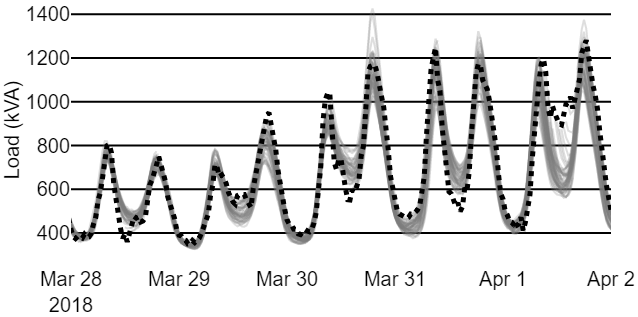
\includegraphics[width=.35\textwidth]{images/easter_2018_all_forecast.png}}
	\caption{Forecasts over the Easter 2018 period.
		The red dashed line is the actual historical load and the forecasts, performed every 30 minutes, are overlaid.
		The single system is able to transition smoothly between holiday and normal periods.}
	\label{fig:easter_forecasts}
\end{figure}

\begin{figure}[htbp]
	\centerline{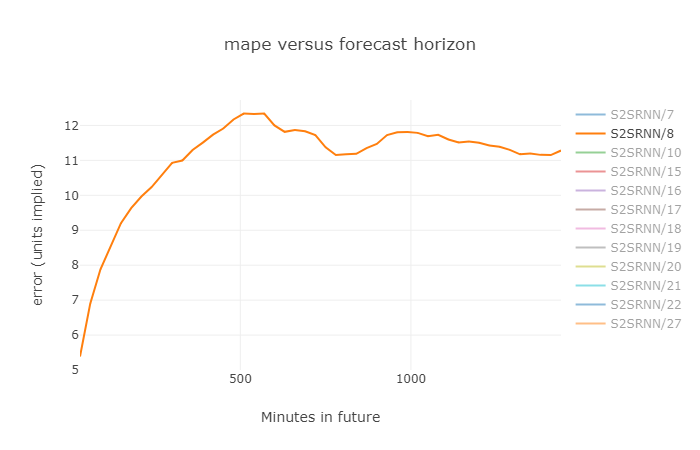
\includegraphics[width=.35\textwidth]{images/bruny_mape.png}}
	\caption{Mean absolute percentage error of each point in the forecast.
		     As expected, the forecaster is generally more accurate for points in the near future.}
	\label{fig:bruny_mape}
\end{figure}

The performance of the forecaster was evaluated on every Easter, Queen's Birthday, and July school holiday from 2015 through 2018 (2018 excludes July).
The results are shown in Figure \ref{fig:bruny_mape}, showing the MAPE as a function of forecast horizon.
As expected, the forecaster achieves high performance on predictions in the near future.
Further, the errors between predicted and actual load resemble white noise, shown in Figure \ref{fig:bruny_hist}.
This is a strong indication that the model has been able to generalize from the training data, as the training data is mostly comprised of normal days.

\begin{figure}[htbp]
	\centerline{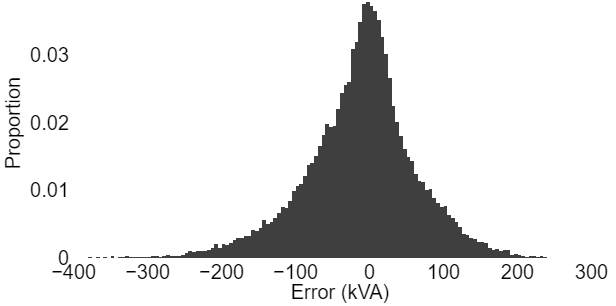
\includegraphics[width=.35\textwidth]{images/errors_histogram.png}}
	\caption{Distribution of forecast error.
		     Notably, this approximates white noise.}
	\label{fig:bruny_hist}
\end{figure}

When implemented live on the Bruny Island distribution network, during the July 2018 school holiday period, the forecaster was observed to reliably forecast large demand peaks.
This enabled the fleet of distributed batteries to be used effectively in providing network support via net demand peak reduction. An accurate forecast, issued early enough in advance of the occurence of the demand peak, was observed to give the batteries adequate time to store energy in the lead up to, and discharge during the demand peak period. In at least one instance over the test period this was sufficient to avoid the island's diesel generator from being used at all, when it otherwise almost certainly would have been required.
Data collected during this peak demand period can be seen in Figure \ref{fig:bruny_nac}.
The upper section shows 24 hours of historical load in black, plus the most recent 24-hour horizon forecast in dashed black (recalculated every five minutes) and all old forecasts in grey.
The lower section shows the battery charge rate, where a negative value of battery charge rate indicates the batteries are supporting the grid.

Typically the generator is switched on when load exceeds 1050 kVA.
During the first peak the graph shows the batteries supplying between 50 and 100 kVA to the island.
Without this support from the batteries it would have been required to use the generator.

\begin{figure}[htbp]
	\centerline{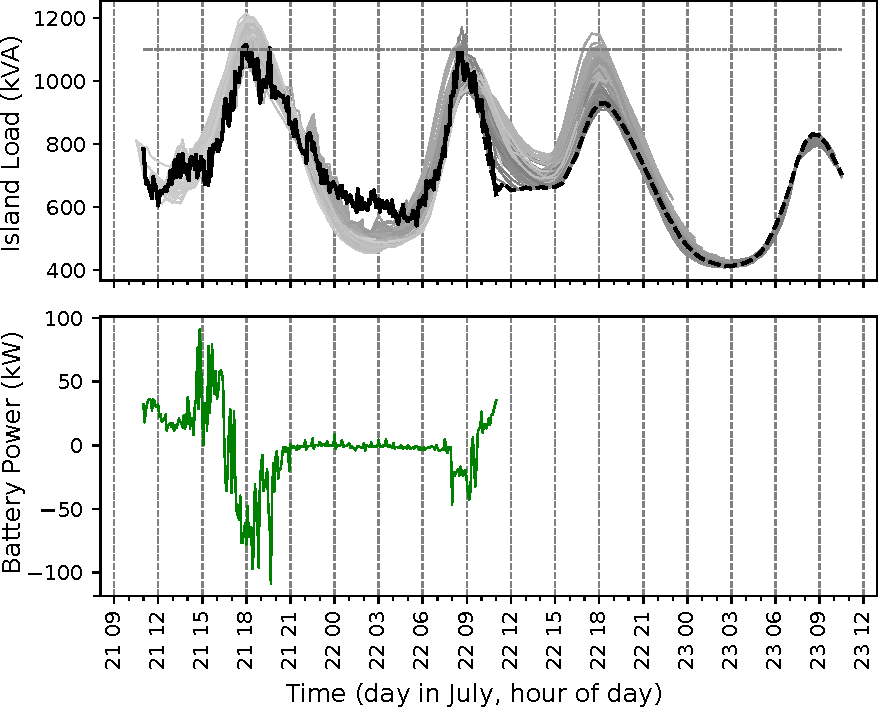
\includegraphics[width=.35\textwidth]{images/bruny_nac.pdf}}
	\caption{The forecaster was able to predict the large peak (top), allowing the batteries to support the island (bottom) and prevent the use of the generator.}
	\label{fig:bruny_nac}
\end{figure}


\section{Conclusion}
Blah Blah the forecaster works.
Used a Transformer model.
Applied to Bruny Island and NAC, helped prevent generator from turning on.
Maybe something about future work?
Reserve some space. Reserve some space. Reserve some space.
Reserve some space. Reserve some space. Reserve some space.
Reserve some space. Reserve some space. Reserve some space.
Reserve some space. Reserve some space. Reserve some space.
Reserve some space. Reserve some space. Reserve some space.
Reserve some space. Reserve some space. Reserve some space.
Reserve some space. Reserve some space. Reserve some space.
Reserve some space. Reserve some space. Reserve some space.
Reserve some space. Reserve some space. Reserve some space.
Reserve some space. Reserve some space. Reserve some space.
Reserve some space. Reserve some space. Reserve some space.
Reserve some space. Reserve some space. Reserve some space.
Reserve some space. Reserve some space. Reserve some space.
Reserve some space. Reserve some space. Reserve some space.
Reserve some space. Reserve some space. Reserve some space.
Reserve some space. Reserve some space. Reserve some space.
Reserve some space. Reserve some space. Reserve some space.
Reserve some space. Reserve some space. Reserve some space.



\section*{Acknowledgment}
This work has been supported by TasNetworks, who also provided network and demand data. It has also been supported by researchers from the ARENA-funded CONSORT Bruny Island Battery Trial.


\bibliographystyle{IEEEtran}
\bibliography{aupec}

\section{TODO} 
\begin{itemize}
	\item Conclusion
	\item Abstract
	\item give a brief over view of tasmanian distribution network in the intro [neg]
	\item CONSORT acronym [neg]
	\item figures right and left to (a) and (b) [neg]
	\item increase the figure text size a lil [neg]
	\item ...Where should not be capitalized in sentences split by equation [neg]
	\item full stops or not in figure captions [neg]
	\item fig gridlines (plotly) [neg]
	\item acknowledgements (probs talk to evan) [neg]
	\item italicise \textit{similar days} maybe to make it clear that they are "a thing" [evan]
	\item make caption of figure \ref{fig:bruny_mape} more independent - specify the period from which the statistics come [evan]
	\item put in new NAC plot [paul]
	\item some conflict between Q,K,V attention and time series length notation.
	\item remove (profile for short) it's a lil stinted
	\item figure \ref{fig:bruny_easter} is pretty hard to view easily. text is too small, probably too many days shown. You may as well use this opportunity to show how the profiles look over just a few days perhaps.. ie give the reader a sense for the difficulty of the problem etc. [evan]
	\item  .[figure \ref{fig:bruny_network}]  there is also a North Bruny A load  that is fed from Feeder A. Prob not too important to make it so accurate.... but just looks a little like there are only two lumped loads on feeder A... no big deal  [evan]
	\item .[figure \ref{fig:easter_forecasts}] it is too hard to see the forecast vs actual for this many days. really need to zoom in I think... text too small on figs too
	\item Explain better why I'm finding similar days, and how I'm using them [evan, paul]
	\item clarify use of future temperature, etc. in similar day selection [paul]
	\item \textbf{PAUL} - if I interpret your comment correctly - the weather forecast is used to find similar days - it's used for the future min and max temperature values. When online, this is done after the program receives the weather forecast as an input.
	\item the description of where the model gets its similar day values from is pretty bad. Needs to be revised [paul]
	\item \textbf{PAUL} - Using all ten years in inference is certainly possible and probably valid. Need to harass a statistician and get their opinion on the validity. Would also require a fair modification to the program :(  currently inference mode IS test mode.
	\item full stop at end of every figure caption. [neg, paul]
	\item expand figure \ref{fig:bruny_easter} to show fewer days. [paul]
	\item reconfigure figure \ref{fig:bruny_network} to consume less vertical space. Could make it horizontal. [paul]
	\item stretch out figure \ref{fig:easter_forecasts} to show fewer days [paul]
	
	
	
	
	
\end{itemize}

\section{Notes questions etc.} 
\begin{itemize}
	\item Notation of layers, in the equations like Equation \ref{dense_layer} I've written $\textbf{Y} = f(\textbf{X})$ but these variables could be interpreted to conflict with the inputs and outputs of the Transformer which are also $\textbf{X}$ and $\textbf{Y}$. Issue?
\end{itemize}

\end{document}
